\documentclass[11pt,dvipdfmx,a4paper]{jsarticle}

\usepackage{amsmath,amssymb}
\usepackage{bm}
\usepackage[dvipdfmx]{graphicx}
\usepackage{physics} % http://mirrors.ibiblio.org/CTAN/macros/latex/contrib/physics/physics.pdf
\usepackage{siunitx} %SI単位を楽に出力
\usepackage{mathtools} %環境の追加
\usepackage{circuitikz} %電気回路をtex中で書く
% \usepackage{caption} %番号なしキャプションを書く
% \usepackage{cancel} %式中に斜線を入れる
% \usepackage{tensor} %テンソルの添え字を書く
% \usepackage{tikz} %図を書く
% \usepackage{ascmac} %四角い枠の中に文章を書く
% \usepackage{float} %figureで[hbp]オプションを使う
% \usepackage{hyperref}  \usepackage{pxjahyper} %ハイパーリンクをつかう
% \usepackage{tablefootnote} %表中に注釈をいれる
% \usepackage[thicklines]{cancel} %数式中の取り消し線
\usepackage[version=4]{mhchem} %化学式の入力
\usepackage{pdfpages}
\usepackage{wrapfig} %文章の回り込み
\usepackage[subrefformat=parens]{subcaption} %(a)図のようにすることができるやつ
\usepackage{here}
\usepackage{mathrsfs} % フォントの追加
\usepackage{url} % url を入れる
\usepackage[margin=15mm]{geometry} %余白の削除
\usepackage{tcolorbox}

\graphicspath{{./image/}}

\begin{document}

%出力したpdfを表紙にするとき
% \includepdf[pages=1,noautoscale=false]{cover.pdf}
% \newpage

%texで表紙を書くとき
\quad\\[35mm]
\centerline{\Huge{\textsf{第 7 回}}}
\quad\\[5mm]
\centerline{\Huge{\textsf{応 用 物 理 学 実 験}}}
\quad\\[5mm]
\begin{table}[h]
	\centering
	\begin{tabular}{| c | c |}
		\hline
		\Huge\textsf{{題目}} & \Huge{\textsf{強誘電体ヒステリシス曲線}} \rule[-5mm]{0mm}{15mm} \\
		\hline
	\end{tabular}
\end{table}
\quad\\[10mm]
\begin{table}[h]
	\centering
	\begin{tabular}{l l}
		\hline
		\LARGE{\textsf{氏\qquad 名}} & \LARGE{\textsf{: 西原 翔}} \rule[0mm]{0mm}{6mm} \\
		\hline
		\LARGE{\textsf{学  籍  番  号}} & \LARGE{\textsf{: 1522068}} \rule[0mm]{0mm}{6mm} \\
		\LARGE{\textsf{学部学科学年}} & \LARGE{\textsf{: 理学部第一部応用物理学科3年}}\\
		\hline
	\end{tabular}
\end{table}
\quad\\[10mm]
\centerline{\LARGE{\textsf{共同実験者:1522064 中井空弥}}}\\[2mm]
% \centerline{\LARGE{\textsf{\qquad\qquad\quad\;\;1522091 宮田祟杜}}}\\[2mm]
% \centerline{\LARGE{\textsf{\qquad\qquad\quad\;\;1522095 村山涼矢}}}\\[2mm]
% \centerline{\LARGE{\textsf{\qquad\qquad\quad\;\;1522B02 中村洸太}}}\\[2mm]
\quad\\[10mm]
\centerline{\LARGE{\textsf{提出年月日:2024年10月24日}}}\\[2mm]
\centerline{\LARGE{\textsf{実験実施日:2024年10月04日}}}\\[2mm]
\centerline{\LARGE{\textsf{\qquad\qquad\quad\;2024年10月11日}}}
\quad\\[10mm]
\centerline{\LARGE{\textsf{東 京 理 科 大 学 理 学 部 第 1 部}}}\\[2mm]
\centerline{\LARGE{\textsf{応 用 物 理 学 教 室}}}

\thispagestyle{empty}
\clearpage
\addtocounter{page}{-1}
\newpage

% \twocolumn

\section{Abstract}
強誘電体はその自発分極の向きによって情報を保存するメモリとしてや、コンデンサとして現在役立てられている。
この強誘電体の自発分極を持つという性質は温度を上げていくといずれ失われ、
自発分極を持たない常誘電体へと相転移する。
誘電体・強誘電体相転移をすることで知られる
\ce{BaTiO_3} (BTO) と \ce{(NH_2CH_2COOH)_3 H_2 SO_4} (TGS) の外部電場に対する電束密度の応答を
室温から相転移温度以上の温度の間で測定した。
BTO は直前の状態に依存して変わるヒステリシス現象を強誘電相・常誘電相、両方において示し、
TGS は強誘電相でのみ示した。
この応答の違いは強誘電性の起源となる仕組みが違うことを表している。
これらの振る舞いを結晶の対称性を反映した自由エネルギーを用いて議論する
Ginzburg-Landau 理論の示す結果と比較した。

\section{Introduction}
強誘電体は電場をかけずとも自発分極を持ち、また外部電場によってその向きを変えることができる。
これはつまり不揮発性メモリとして利用することができる。
またこれを用いたコンデンサはサイズに対する静電容量が大きくコンデンサとしての用途も期待できる。
さらに、強誘電体はその結晶構造によるところが大きく、ひずみよって分極が変わる。
これより圧力のセンサーとしても使うことができる素材である。
そのためこれまでにも強誘電体の性質やこれを応用したデバイスの研究が広く行われてきた。

そうした強誘電体は温度を上げていくと自発分極を持つという性質を失った常誘電体へと変化する。
この相転移の様子をかけた電場への応答という点から測定していく。

今回、変位型強誘電体の代表として BTO, 規則不規則型強誘電体の代表として TGS を測定した。
前者はセラミックコンデンサとして、後者は圧電センサーとして利用されている素材である。
これら素材の結晶学的な性質をまとめる。

\begin{figure}[H]
    \centering
    \begin{minipage}[t]{0.48\columnwidth}
        \centering
        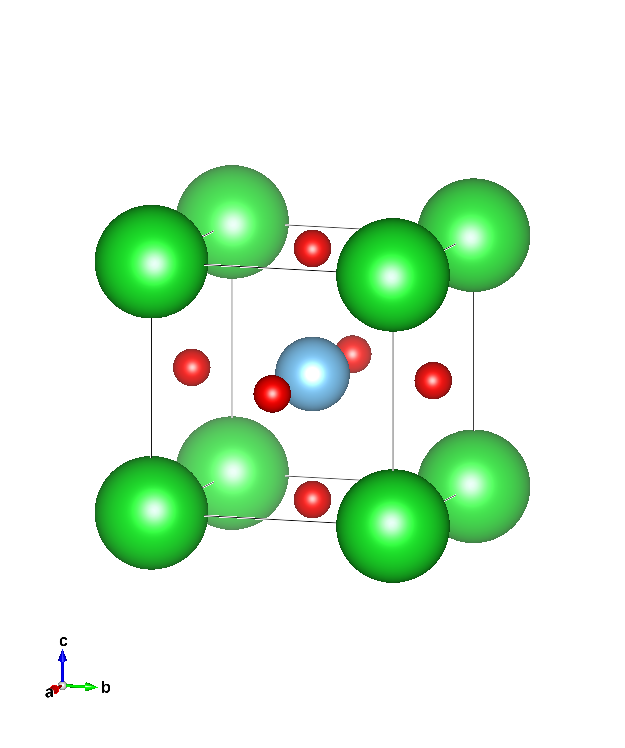
\includegraphics[width = \columnwidth]{structure/BTO.png}
        \subcaption{\ce{BaTiO_3}の立方晶ペロブスカイト構造。
        空間群は $Pm\bar{3}m$, 格子定数は a = 4.04 \AA.
        緑色が Ba, 青色が Ti, 赤色が O を表している。}
        \label{structure:BTO}
    \end{minipage}
    \begin{minipage}[t]{0.48\columnwidth}
        \centering
        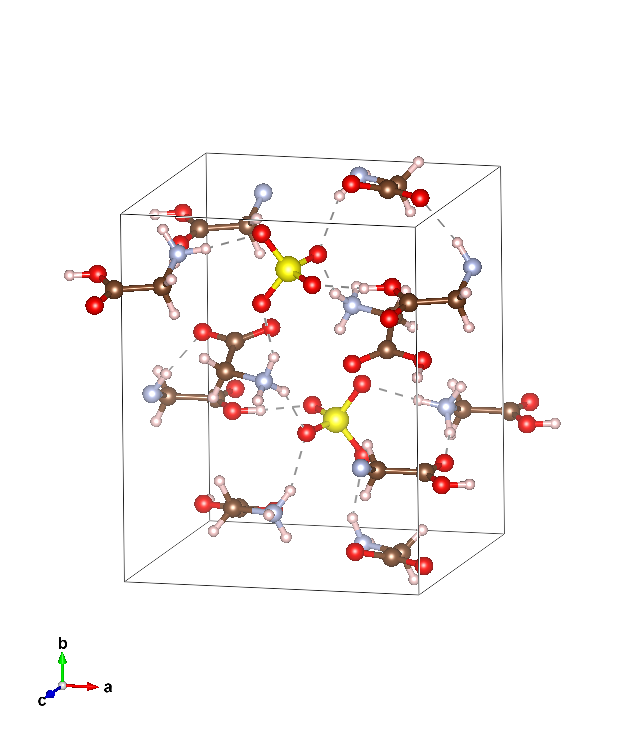
\includegraphics[width = \columnwidth]{structure/TGS.png}
        \subcaption{\ce{(NH_2CH_2COOH)_3 H_2SO_4}の構造。
        空間群は $P2_1$, 格子定数は a = 9.44 \AA, b = 12.63 \AA, c = 5.71 \AA, $\beta$ = 110\si{\degree}.
        cif データ\cite{cif:7128310} をもとに作成した。
        黄色と赤色の四面体が硫酸イオン、
        その他の黒色と青色からなる構造がグリシンである。}
        \label{structure:TGS}
    \end{minipage}
    \caption{今回測定した試料の結晶構造。VESTA\cite{VESTA}を用いて作成した。}
\end{figure}

\subsection{試料の結晶構造}
\subsubsection*{\ce{BaTiO_3}}
\ce{BaTiO_3} はペロブスカイト型酸化物 \ce{ABO_3} の一種であり、BTO と略される。
理想的な立方晶ペロブスカイトの構造は金属原子 A が単位胞の各頂点、
金属原子 B が単位胞の体心位置、酸素 O が面心位置を占有しているような構造である(図\ref{structure:BTO})。
A 原子と B 原子を置換することで格子定数や電子密度を変えることができ、
物性を変え様々な機能を持たせることができる構造である。
ただ、構成する金属原子や環境の温度・圧力によっては \ce{BO_6} の正八面体が傾いたり歪みが生じ、
対称性の異なる結晶構造になる。
BTO は絶対零度の基底状態から温度を上げていくと順に
菱面体晶$(R3m)$, 斜方晶$(Amm2)$,
正方晶$(P4mm)$,
立方晶$(Pm\bar{3}m)$へと変化する。
ここでの括弧内は空間群を表している\footnote{空間群については付録に乗せた。}。

\subsection*{\ce{(NH_2CH_2COOH)_3 H_2SO_4}}
\ce{(NH_2CH_2COOH)_3 SO_4} は TGS と略され、アミノ酸であるグリシン\ce{NH_2CH_2COOH} 3つと硫酸\ce{H_2SO_4}が集まったものである。(図\ref{structure:TGS})。
空間群は $P2_1$, 格子定数は a = 9.44 \AA, b = 12.63 \AA, c = 5.71 \AA, $\beta$ = 110\si{\degree} の単斜晶の結晶である。
これは b 軸方向に沿って硫酸イオンとグリシンの層、アミノ基にプロトンがくっついているグリシン2つの層が水素結合によって交互に積層している構造である。


\section{Methods}
\begin{wrapfigure}{r}[0pt]{0.35\columnwidth}
    \centering
    \begin{circuitikz}
        \draw (0, 0)
            to[tV, v=$V_i$] (0, 2)
            to[short] (2, 2)
            to[C=$C_x$] (2, 1)
            to[C=$C_s$] (2, 0)
            to[short] (0, 0);
        % \draw (2, 1)
        %     to[short, -o] (3, 1)
        %     node[anchor=west]{Ch. 2};
        \draw (-0.5, 1.5)
            node[anchor=south]{50Hz};
        \draw(0,0) to node[ground]{} ++(0,0);
    \end{circuitikz}
    \caption{電場に対する試料の電束密度の応答を調べる回路(Sawyer-Tower 法)。
    $C_s$がサンプルの静電容量、$C_x$は標準コンデンサの静電容量。
    入力は 50 Hz の三角波。オシロスコープの Ch.1 で入力三角波の電圧を、
    Ch.2 で$C_s$の両端の電圧差を測定することで試料にかけた電場\(E\)に対する応答である電束密度\(D\)を測定できる。}
    \label{fig:circuit}
\end{wrapfigure}
試料に\(E\)の電場をかけたときの試料中の電束密度\(D_x\)の大きさを測定する回路の模式図は図\ref{fig:circuit}である。
実際にはアンプ等が入っているが物理量の測定の仕組みにかかわる部分を抜き出してある。
\(C_x\)がサンプルの静電容量、\(C_s\)が標準コンデンサの静電容量で\(C_s\gg C_x\)になるように標準コンデンサを選んである。
50 Hz の三角波を入力として、これを記録するためにオシロスコープの Ch.1 で記録する。
この 50 Hz の周期的な入力ではあるが、誘電体の配向分極と共鳴する振動数は 1kHz 程度のオーダーである(2OB 実験:複素インピーダンス測定)
のでこの入力は直流入力だとみなすことができる。
また、\(C_s\)の両端の電圧差をオシロスコープの Ch.2 で記録をする。
このとき、試料にかかる電圧はオシロスコープの各チャンネルに入力される電圧を\(V_{\text{Ch.1}}, V_{\text{Ch.2}}\)とすると、
コンデンサ回路の電荷保存則より試料にかかる電圧\(V_x\)と標準コンデンサにかかる電圧\(V_{\text{Ch.2}}\)は
\begin{align}
    V_x &= \frac{C_s}{C_s+C_x}V_{\text{Ch.1}} \simeq V_{\text{Ch.1}}\\
    V_{\text{Ch.2}} &= \frac{C_x}{C_s+C_x}V_{\text{Ch.1}} \simeq \frac{C_x}{C_s}V_x
\end{align}
というように書ける。ここでコンデンサ表面の電荷と電束密度の間のガウスの法則により、
平行版コンデンサの面積を\(A\)として
\begin{align}
    C_x V_x = Q_x = D_x A
\end{align}
というように書ける。
そして試料にかかっている電場の大きさは平行版コンデンサの厚さを\(d\)として\(E = V/d\)と書ける。
これらをまとめると
\begin{align}
    E = \frac{1}{d}V_{\text{Ch.1}}, \qquad
    D_x = \frac{C_s}{A}V_{\text{Ch.2}}
\end{align}
というようになり、オシロスコープのXYモードで表示させることで
試料に電場\(E\)をかけたときの試料中の電束密度\(D_x\)の関係を表示・記録することができるのがわかる。

電束密度\(D_x\)の温度依存性を見るため、実際の系では\(C_x\)は熱電対温度計と共に炉の中に入れ測定した。


\section{Results}

\section{Discussion}
\subsection{強誘電・常誘電相転移の機構}
BTOでの相転移はペロブスカイトの構造による格子振動とクーロン相互作用の結合による構造の不安定化によるものである。
%仮置き
格子振動は電荷の偏りを生じる光学モードと偏りを生じない音響モードの2つがある。
光学モードにおける電荷の偏りはつまり分極と解釈できる。
分極は外部電場と結びつくため云々。

\section{Conclusion}


\bibliographystyle{junsrt}
\bibliography{reference}
\nocite{*}

% \appendix
% \section{点群・空間群}
% 結晶に対称性があるといったとき、
% それは結晶を回転させたり、鏡映しにしたりしてもその格子点の配置が変わらないということによって特徴づけできる。
% つまりある操作が与えられたときにその結晶の格子点の配置が変わるか変わらないかで結晶を分類することができる。

% 結晶全体を平行移動させる並進操作によって

% % 結晶を対称性によって分類し、その性質を見ていくのに数学における群論という代数が適している。
% % 集合\(G\)とその上の二項演算\(\cdot\)の組が群であるとは次の3つの条件を満たすことをいう。
% % \begin{itemize}
% %     \item 任意の\(G\)の元 \(g,\,h,\,k\)に対して\(g\cdot(h\cdotk) = (g\cdot h) \cdot k\)
% %     \item 任意の\(G\)の元 \(g\) であっても \(e\cdot g = g\cdot e = g\)を満たすような\(G\)の元\(e\)が存在する。
% %     \item 任意の\(G\)の元 \(g\) に対して \(g \cdot g^{-1} = g^{-1}\cdot g = e\)となるような\(G\)の元\(g^{-1}\)が存在する。
% % \end{itemize}
% % 群の例として、整数\(\mathbb{Z}\)は加法に関して群であり、
% % 逆行列が非負の\(n\times n\)行列全体\(GL(n,\mathbb{R})\)は行列の積に関して群である。
% これを


% \section{結晶の対称性と Ginzburg-Landau 理論}

\end{document}